\documentclass[12pt, a4paper,  nobibnotes]{article}

%%%%%%%%%%%%%%%%%
% Configuration %
%%%%%%%%%%%%%%%%%
\usepackage{amsmath}
% If magyar is wanted
\usepackage[T1]{fontenc}
\usepackage[utf8]{inputenc}
\usepackage{fixltx2e}
\usepackage{multirow}
\usepackage{url}
\usepackage{amsfonts}
\usepackage{amsthm}
\usepackage{mathtools}
\usepackage{amssymb}

\usepackage[dvipsnames]{xcolor}
\newcommand{\red}[1]{\textcolor{red}{#1}}

\usepackage{setspace}
\onehalfspacing

% Nice algorithms
\usepackage{algorithm}
\usepackage{algpseudocode}

% Margins 
\usepackage{anysize}
\marginsize{1.64cm}{2.0cm}{1.2cm}{2.4cm} %\left right top bottom

% Multiple languages
\usepackage[english,magyar]{babel}

% using circled symbols
\usepackage{tikz}
\newcommand*\circled[1]{
    \tikz[baseline=(char.base)]{
        \node[shape=circle,draw,inner sep=2pt] (char) {#1}
    }
}

\newcommand{\op}[1]{\hat{#1}}
\newcommand{\ketbra}[2]{|#1\rangle\langle#2|}
\newcommand{\Ketbra}[2]{\left|#1\right\rangle \left\langle#2\right|}

%%%% Some things for fancier look %%%%
\frenchspacing
\setlength{\parskip}{2ex}
\setlength{\headsep}{0,4cm}
\setlength{\headheight}{4pt}

% fej- es lábléc
\usepackage{fancyhdr}
\usepackage{fancyref}
\usepackage{fancyvrb}
\pagestyle{fancy}

\renewcommand{\headrulewidth}{0,05pt}
\renewcommand{\footrulewidth}{0pt}


\fancyhf{}
\fancyhead[RE]{{ \nouppercase{\leftmark}} }
\fancyhead[LO]{{ \nouppercase{\leftmark}} }
\cfoot{--~\thepage~--}
%%%%%%%%%

% For quantum circuits.
\usetikzlibrary{quantikz}

\usetikzlibrary{fadings}
\usetikzlibrary{patterns}
\usetikzlibrary{shadows.blur}
\usetikzlibrary{shapes}

% Here you can configure the layout
\usepackage{geometry}
\geometry{top=1cm, bottom=1cm, left=1.25cm,right=1.25cm, includehead, includefoot}
\setlength{\columnsep}{7mm} % Column separation width

\usepackage{graphicx}

%\usepackage{gensymb}
\usepackage{float}

% For bra-ket notation
\usepackage{braket}

% To have a good appendix
\usepackage[toc,page]{appendix}

\usepackage{abstract}
\renewcommand{\abstractnamefont}{\normalfont\bfseries}
\renewcommand{\abstracttextfont}{\normalfont\small\itshape}
\usepackage{lipsum}

%%%%%%%%%%%%%%%%%%%
% Custom commands %
%%%%%%%%%%%%%%%%%%%
\newcommand{\bb}[1]{\mathbf{#1}}
\newcommand{\dd}{\mathrm{d}}
\newcommand{\Tr}[1]{\mathrm{Tr}\left[#1\right]}
\newcommand{\Sp}[1]{\mathrm{Sp}\left[{#1}\right]}

\newtheorem*{theorem*}{Theorem}
\newtheorem*{definition*}{Definition}
\newtheorem*{example*}{Example}
\newtheorem*{problem*}{Problem}
\newtheorem*{remark*}{Remark}
\newtheorem*{statement*}{Statement}

\newtheorem{theorem}{Theorem}
\newtheorem{definition}{Definition}
\newtheorem{example}{Example}
\newtheorem{problem}{Problem}
\newtheorem{remark}{Remark}
\newtheorem{statement}{Statement}

\usepackage[square,numbers]{natbib}
\bibliographystyle{unsrtnat} %{abbrvnat}

%% COMMENTS
\newcommand{\nd}[1]{\textcolor{Aquamarine}{\textbf{[Dani: #1]}}}

% Hyperref should be generally the last package to load
% Any configuration that should be done before the end of the preamble:

\usepackage{hyperref}
\hypersetup{colorlinks=true, urlcolor=blue, linkcolor=blue, citecolor=blue}

%%%%%%%%%%%%%%%%%%%%%%%%%%%%%%%%%%%%%%%%%%%%%%%%%%%%%%%%%%%%%
%                    BEGIN    DOCUMENT                      % 
%%%%%%%%%%%%%%%%%%%%%%%%%%%%%%%%%%%%%%%%%%%%%%%%%%%%%%%%%%%%%

\begin{document}
\selectlanguage{english}
\begin{center}
\vspace*{5.0cm}
\LARGE{Experimenting with machine learning algorithms on quantum computers}\\
\vspace{2.0cm}
\large{Nagy Dániel$^1$}\\
\vspace{2.0cm}
\large{
    $^1$Institute for Physics, Eötvös Loránd University, H-1117, Pázmány Péter sétány 1/A. Budapest, Hungary\\%
    \vspace{5.0cm}
    Created on December 1, 2019\\
    \vspace{1.0cm}
    Last update: \today
}
\end{center}
\thispagestyle{empty} %% No fancy
\newpage

\begin{center}
    \textbf{Abstract}\\
    \par A modern számítástechnika jelentős eredményei közé tartozik a gépi
    tanulás és mesterséges intelligancia alapvető algoritmusainak kifejlesztése és ezek 
    hasznosságának tesztelése különböző feladatokon. Ugyanakkor az elmúlt években a 
    kvantumszámítás is jelentős fejlődésen ment keresztül, olyannyira, hogy 2019-ben a Google kísérleti
    csapatának sikerült demonstrálnia a kvantumfölényt. A munka során megvizsgáljuk a két terület átfedéséből 
    származó lehetőségeket: klasszikus adatok kvantumos feldolgozását illetve a klasszikus
    gépi tanulás segítségével történő kvantumos hibajavítást.
\end{center}
\thispagestyle{empty} %% No fancy
\newpage

\selectlanguage{magyar}
\begin{center}
\vspace*{5.0cm}
\LARGE{Gépi tanulási algoritmusok vizsgálata kvantumszámítógépeken}\\
\vspace{2.0cm}
\large{Nagy Dániel$^1$}\\
\vspace{2.0cm}
\large{
    $^1$Eötvös Loránd Tudományegyetem, Fizika Intézet, H-1117, Pázmány Péter sétány 1/A. Budapest, Magyarország\\%
    \vspace{5.0cm}
    Elkezdve: December 1, 2019\\
    \vspace{1.0cm}
    Utolsó frissítés: \today
}
\end{center}
\thispagestyle{empty} %% No fancy
\newpage


\begin{center}
    \textbf{Kivonat}\\
    \par A modern számítástechnika jelentős eredményei közé tartozik a gépi
    tanulás és mesterséges intelligancia alapvető algoritmusainak kifejlesztése és ezek 
    hasznosságának tesztelése különböző feladatokon. Ugyanakkor az elmúlt években a 
    kvantumszámítás is jelentős fejlődésen ment keresztül, olyannyira, hogy 2019-ben a Google kísérleti
    csapatának sikerült demonstrálnia a kvantumfölényt. A munka során megvizsgáljuk a két terület átfedéséből 
    származó lehetőségeket: klasszikus adatok kvantumos feldolgozását illetve a klasszikus
    gépi tanulás segítségével történő kvantumos hibajavítást.
\end{center}
\thispagestyle{empty} %% No fancy
\newpage

\begin{center}
    \nd{Acknowledgement}
\end{center}

\selectlanguage{english}
% Add a link target to the TOC itself
\addtocontents{toc}{\protect\hypertarget{toc}{}}
\thispagestyle{empty}
\tableofcontents
\newpage

\thispagestyle{empty}
\listoffigures
\newpage

\section{Introduction}
Quantum computing is probably the most promising emerging technology with many possible applications across
all domains of science and business. The idea of quantum computing was first proposed by Richard P. Feynman
as a method to simulate quantum mechanics. Since the size of the Hilbert-space grows exponentially with
the complexity of the quantum system, and thus the calculations become intractable on any classical
computer, Feynmans idea was to simulate quantum physics on devices that behave themselves according to 
the rules of quantum physics.
\par
Soon after Feynmans proposal, scientists became to establish the theoretical background of quantum
information and quantum computing. Some of the quantum algorithms are proven to have an 
advantage over any known classical algorithm. One of the first such quantum algorithm is 
the Deutsch-Jozsa algorithm \cite{DeutschJozsa1992}, which decides if a binary function $f$ 
is balanced or constant. Probably the most notable quantum algorithm was proposed by Peter W. Shor 
in 1994, which is a polynomial-time quantum algorithm for factoring large integers \cite{Shor1994}.
This is the first quantum algorithm with a real-life application, because most of the public-key
cryptosystems could be broken with an efficient algorithm for integer factoring. 
Another important quantum algorithm is the Grover's algorithm proposed by Lov K. Grover in 1996 for
searching an unordered database \cite{Grover1996}. While the best known classical algorithm 
for searching unordered databases runs in $O(N)$ time, Grover's algorithm solves this problem
with $O(\sqrt N)$ oracle queries. Beyond quantum algorithms, many quantum-inspired algorithms were 
discovered \cite{Tang2019,Ding2019QuantumInspiredSVM,ArrazolaQuantumInspired2019}.

\cite{KLMScheme}, \cite{XanaduBlueprint}, \cite{PsiQuantumFBQC}
\nd{cite: Xanadu paper, Photonic Supremacy paper, PsiQuantum Fusion-Based QC}


\section{Quantum Computing with continuous variables}
In this chapter, we introduce the mathematical formalism used in the description of 
continuous-variable (CV) quantum computing. This formalism is quite different from the 
formalism used in qubit-based quantum computing literature, mostly because
CV systems have infinite degrees of freedom. 
We assume that the reader has basic knowledge of quantum mechanics, Hilbert-spaces, density
matrices, braket notation, etc. Some of this basic mathematical background is covered in appendix
\ref{appendix:mathematical-preliminaries}. 
CV systems have infinite degrees of freedom, and therefore the corresponding Hilbert-space is of infinite dimensions. 
Such systems can be modeled by $M$ harmonic oscillators, which are usually called \textit{modes}. 
% each having a Hilbert-space $\mathcal H_k$. 
With $H_k$ denoting the Hilbert-space of the $k$th mode, the Hilbert-space of the full CV system is their direct sum:
\begin{equation}
    \mathcal H = \bigoplus\limits_{k=1}^M\mathcal H_k.
\end{equation}
The Hamiltonian of mode $j$ can be described by introducing bosonic creation and annihilation operators $a_j^\dagger$ and $a_j$, obeying the following canonical commutation relations:
\begin{align}
    \left[\op a_j, \op a_k^\dagger \right] = \delta_{jk}, & \left[\op a_j^\dagger, \op a_k^\dagger\right] = \left[\op a_j, \op a_k\right] = 0.
\end{align}
The effect of the creation and annihilation operators on the Fock space can be described by the 
following identities:
\begin{align}
    \begin{split}
    &\op a_k^{\dagger} \ket{n_1, \dots, n_k, \dots} = \sqrt{1+n_k}\ket{n_1, \dots, n_k + 1, \dots} \\
    &\op a_k \ket{n_1, \dots, n_k, \dots} = \sqrt{n_k} \ket{n_1, \dots, n_k - 1, \dots} \\
    \end{split}
\end{align}
We also introduce the number operator $\op n_j=\op a_j^\dagger \op a_k$:
\begin{align}
 &\op a_k^\dagger \op a_k |n_1, ..., n_k, ... \rangle = \op n_k |n_1, ..., n_k, ... \rangle = n_k |n_1, ..., n_k, ... \rangle
\end{align}
Each of the single-mode Hilbert-space $\mathcal H_k$ is an infinite-dimensional Fock-space spanned by the eigenvectors 
of the number operator $\op n_k = \op a_k^\dagger \op a_k$ labeled $\{\ket{n}\}_k$.
It is often useful to introduce the canonical position operators $X_j$ and momentum operators $P_j$ which are related to the creation and annihilation operators
by the following transformations:
\begin{align}
  \op X_k &= \frac{\op a_k+\op a_k^\dagger}{\sqrt{2}}  & \op a_k &= \frac{\op X_k + i\op P_k}{\sqrt{2}}  \\ 
  \op P_k &= \frac{\op a_k-\op a_k^\dagger}{i\sqrt{2}} & \op a_k^\dagger &= \frac{\op X_k - i\op P_k}{\sqrt{2}}
   \label{eq:jwtransform}
\end{align}
Operators $\op X_k$ and $\op P_k$ are called quadrature operators. Following the notation often used in literature, we group these operators into a vector 
\begin{equation}
    \mathbf R^\top = (\op X_1, \op P_1, \op X_2, \op P_2, ..., \op X_k, \op P_k, ..., \op X_M, \op P_M)
    \label{eq:xidef}
\end{equation}
We can calculate the commutators $\left[\mathbf R_k,\mathbf R_l\right]$ by introducing a symplectic form $\pmb\Omega$ as
\begin{equation}
    \pmb\Omega = \bigoplus\limits_{j=1}^{M}\pmb\omega,~\pmb\omega = 
    \begin{pmatrix}
    0 & 1 \\
    -1 & 0
    \end{pmatrix}.
\end{equation}
Using this notation, we can write
\begin{equation}
    \left[\mathbf R_k,\mathbf R_l\right] = i\pmb\Omega_{kl}
\end{equation}

Apart from the Fock-basis, there is another useful alternative basis, the basis of \textit{coherent states},
which are eigenstates of the annihillation operator $\op a_k$:
\begin{equation}
    \op a_k \ket{\alpha}_k = \alpha\ket{\alpha}_k,
\end{equation}
with $\alpha\in\mathbb C$. From definition this, we can derive that the Fock-basis expansion of 
the coherent state $\ket\alpha_k$ is
\begin{equation}
    \ket\alpha_k = e^{-\frac{1}{2}|\alpha|^2}\sum\limits_{n=1}^\infty \frac{\alpha^n}{\sqrt{n!}}\ket n_k.
\end{equation}
The derivation of the above formula is explained in detail in appendix \ref{appendix:coherent}. By introducing 
the single-mode Weyl-displacement operator 
\begin{equation}
    \op D_k(\alpha) = e^{\alpha\op a^\dagger_k - \alpha^*\op a_k},
    \label{eq:singlemode-weyl}
\end{equation}
we can create coherent states from the vacuum state: $\ket\alpha_k = \op D_k(\alpha)\ket 0_k$. Of 
course, we can define multimode coherent states 
\begin{equation}
    \ket{\alpha_1}_1 \otimes \ket{\alpha_2}_2 \otimes \cdots \otimes \ket{\alpha_N}_N \equiv \ket{\pmb\xi} = \op D(\pmb\xi) \ket 0,
\end{equation}
where $\op D(\pmb\xi)$ is the multi-mode Weyl-displacement operator defined as
\begin{equation}
    \op D(\pmb\xi) = e^{i\mathbf R^\top\pmb\Omega\pmb\xi}, ~ \pmb\xi \in \mathbb R^{2N}.
    \label{eq:multimode-weyl}
\end{equation}
For a single mode, 
\begin{equation}
    \op D_k(\pmb\xi) = \op D_k\left(\begin{matrix}
        \xi_1 \\ \xi_2
    \end{matrix}\right)
    = e^{i(\xi_2 \op X_k - \xi_1 \op P_k)},\,\textrm{if we set}\,\left(\begin{matrix}
        \xi_1 \\ \xi_2
    \end{matrix}\right) = \frac{1}{\sqrt 2}\left(\begin{matrix}
        \textrm{Re}(\alpha_k) \\ \textrm{Im}(\alpha_k)
    \end{matrix}\right),
\end{equation}
equation \ref{eq:multimode-weyl} reproduces equation \ref{eq:singlemode-weyl}. The introduction
of the Weyl-displacement operator is necessary to carry out the phase-space description
of CV-systems, which we will do in the next chapter.

\subsection{Phase-space description}
\label{sec:phasespace}
The description of CV quantum systems with the help of canonical creation and annihillation operators in 
the Fock-basis is equivalent to the description of these systems in the quadrature basis, 
which is called the phase-space description. The phase-space description is useful, 
because it makes possible to calculate quantities easier than it would be in the Fock-basis description.

A CV quantum state $\op\rho$ can be descibed in Fock-space by an infinite-sized matrix. This is 
problematic if we want to carry out actual calculations or simulate such systems. However, 
phase-space description can be used to deal with these problems. Instead of giving the elements
of the density matrix $\op\rho$, we can use the \textit{s-ordered characteristic functions} 
(see \cite{Adesso2014}) to describe the state:
\begin{equation}
    \chi_{\op \rho}^s(\pmb\xi) = \Tr{\op\rho\op D(\pmb\xi)}e^{s||\pmb\xi||^2/2},~\pmb\xi\in\mathbb R^{2N}.
\end{equation}
The $2N$-dimensional vectors $\pmb\xi$ lie in the \textit{quantum phase-space} $\Gamma$. The 
quantum phase-space $\Gamma=(\mathbb R^{2N}, \pmb\Omega)$ is a real $2N$-dimensional space 
equipped with the symplectic form $\pmb\Omega$. While $\Gamma$ is the quantum phase-space of the 
$N$-mode system, it can be decomposed into a direct sum of single-mode quantum phase spaces:
\begin{equation}
    \Gamma = \bigoplus\limits_{k=1}^N\Gamma_k,
\end{equation}
where $\Gamma_k=(\mathbb R^2, \pmb\omega)$ are the $2$-dimensional phase spaces associated with 
the $k$th mode. Unlike in classical mechanics, where a state of the system is a single point 
in its phase-space, quantum states are not single points, but a region in the phase space. This 
is a consequence of the Heisenberg uncertainty principle, and the phase-space region 
corresponding to a state depends on the product of the uncertainties of the 
quadrature operators.
\par
By applying a Fourier-transform to the s-ordered characteristic function, we 
can define a corresponding quasi-probability function:
\begin{equation}
    W_{\op\rho}^s(\pmb\xi) = \frac{1}{\pi^2}\int_{\mathbb R^{2N}}\chi_{\op\rho}^s
    e^{i\pmb\kappa^\top\pmb\Omega\pmb\xi} \dd^{2N}\pmb\kappa.
\end{equation}
$W_{\op\rho}^s(\pmb\xi)$ are called quasi-probabilities, because they sum up to
$1$, but they can have negative values or even be singular in some cases. 
There are a bunch of notable quasi-probability distributions associated to 
a state $\op\rho$: for $s=-1$, 
\begin{equation}
    W_{\op\rho}^{-1} = \frac{1}{\pi}\bra{\pmb\xi}\op\rho\ket{\pmb\xi}
\end{equation}
is called the Husimi Q-function, and for $s=1$, we have the so called P-representation or P-function,
which is the representation of $\op\rho$ in the coherent basis:
\begin{equation}
    \op\rho = \int_{\mathbb R^{2N}} W_{\op\rho}^1(\pmb\xi)\ketbra{\pmb\xi}{\pmb\xi}\dd^{2N}\pmb\xi.
\end{equation}
Perhaps the most important quasiprobability is the $s=0$ case, for which $W^{0}_{\op\rho}\equiv W_{\op\rho}$
is called the \textit{Wigner-function}, and $\chi_{\op\rho}^{0}\equiv \chi_{\op\rho}$ is simply called
the characteristic function.
The Wigner-function can be expressed in the quadrature-basis, namely the basis spanned by 
the eigenvectors of the $\op X_j$ operators (the vectors satisfying $\op X_j=X_j\ket{\mathbf x}$), 
which we will denote $\ket{\mathbf x}$:
\begin{equation}
    W_{\op\rho}(\mathbf x, \mathbf p) = \frac{1}{\pi^N}\int_{\mathbb R^N}\bra{\mathbf x + \mathbf y}
    \op\rho \ket{\mathbf x-\mathbf y}e^{-2i\mathbf p\mathbf y}\dd^{N}\mathbf y
\end{equation}
The Wigner-function is normalized, i.e
\begin{equation}
    \int_{\mathbb R^{2N}}W_{\op\rho}(\mathbf x, \mathbf p) \dd^{N}\mathbf x \dd^{N}\mathbf p = \Tr{\op \rho} = \chi_{\op\rho}(0) = 1,
\end{equation}
and it can be used to calculate the \textit{purity} of the state $\mu_{\op\rho}$:
\begin{equation}
    \mu_{\op\rho} = \Tr{\op\rho^2} = (2\pi)^N \int_{\mathbb R^{2N}}\left(W_{\op\rho}(\mathbf x, \mathbf p)\right)^2 \dd^{N}\mathbf x \dd^{N}\mathbf p
    = \int_{\mathbb R^{2N}} |\chi_{\op\rho}(\pmb\xi)|^2 \dd^{2N}\pmb\xi.
\end{equation}
The Wigner-function also can be used to calculate expectation values of the quadrature operators, 
for example $\langle X_1 \rangle$ can be calculated by marginalizing over all other variables, 
that is,
\begin{equation}
    \langle X_1 \rangle = \int_{\mathbb R^{2N-1}} W_{\op\rho}(\mathbf x, \mathbf p) \dd p_1 \cdots \dd p_N \dd x_2 \cdots \dd x_N.
\end{equation}
\nd{Write about different quantum gates.}
\nd{Write about homodyne measurements, heterodyne measurements and photon number-resolving measurements}
\subsection{CV quantum gates}
In this section we present the most important quantum gates used in continuous variable 
systems. We follow the notation also used in the documentation of Strawerry Fields \cite{Killoran2019strawberryfields,StrawberryFieldsDocumentation}.
Some of the gates are Gaussian, others are non-Gaussian, again some of them 
are expressed in terms of canonical creation and annihilation operators, others are expressed 
in terms of the quadrature operators.

In the visual representations of CV quantum circuits,
wires represent photon carriers which are typically integrated waveguides on a 
photonic integrated circuit, while boxes represent the device realizing the corresponding
transformation on the quantum state.

\par \textbf{Displacement.}
\begin{figure}[H]
    \centering
    \includegraphics[width=0.25\textwidth]{figures/displacement.pdf}
\end{figure}

\begin{equation}
     D(\alpha) = e^{\alpha \op a^\dagger - \alpha^* \op a} 
      = \exp\left[r\left(e^{i\phi}\op a^\dagger - e^{-i\phi}\op a \right)\right],
\end{equation}
with $\alpha = re^{i\phi} \in\mathbb{C},\, r\geq 0,\, \phi\in [0,2\pi)$.
\par \textbf{Rotation.}
\begin{figure}[H]
    \centering
    \includegraphics[width=0.25\textwidth]{figures/rotation.pdf}
\end{figure}

\begin{equation}
     R(\phi) = e^{i\phi\op a^\dagger \op a} = \exp\left[\frac{\phi}{2}\left(\frac{\op X^2 + \op P^2}{\hbar}-\op I\right)\right]
\end{equation}


\par \textbf{Squeezing.}
\begin{figure}[H]
    \centering
    \includegraphics[width=0.25\textwidth]{figures/squeezing.pdf}
\end{figure}

\begin{equation}
     S(z) = \exp\left[ \frac{1}{2}\left( z^*\op a^2 - z \op a^{\dagger^2} \right) \right]
     = \exp\left[ \frac{r}{2}\left( e^{-i\phi}\op a^2 - e^{i\phi} \op a^{\dagger^2} \right) \right],
\end{equation}
with $z = re^{i\phi} \in\mathbb{C},\, r\geq 0,\, \phi\in [0,2\pi)$.

\section{Machine learning}
\label{sec:ml-intro}

Machine learning is simply said, a new paradigm in software development. Traditional software have
a predefined behaviour, which does not change over time. In contrast, machine learning models
are iteratively "trained" i.e. updated to achieve better performance by the use of data. These algorithms
are designed to learn patterns from the data available and update themselves with new experience.
Although, there are a lot of machine learning algorithms, they usually fit into one of the following three 
main classes:
\begin{itemize}
    \item \textbf{Supervised Learning}. Supervised Learning (SL) algorithms need labeled data, and
    based on the input-output pairs previously seen by the algorithm, it learns to produce
    correct outputs for previously unseen inputs. A very basic example of supervised learning 
    is the linear regression or support vector machines \nd{ref?} for classification, but there are a lot of complex models like CNNs for image classification
    \nd{ref?}, which are trained in a supervised manner.  
    \item \textbf{Unsupervised Learning}. Unsupervised Learning (UL) does not require labeled data, instead
    of that, it is trying to learn from a lot of unlabeled data points. These algorithms include a bunch
    of clustering methods, like k-means \nd{ref?}, or mixture models \nd{ref?}. Another example of unsupervised
    learning is latent variables or distributions for feature extraction or data denoising. A great example 
    of latent distribution learning are Variational Autencoders \cite{VAEPaper} which have bean adobted 
    for a variety of tasks.
    \item \textbf{Reinforcement Learning}. Reinforcement Learning (RL) is very different from the previously
    mentioned two classes of machine learning method. In RL the goal is not to learn from a given set of 
    data, but rather to solve a specific task in an environment. In RL, an \textit{agent} learns to 
    perform a task by observing the state (or some subspace of the state) of the surrounding environment,
    and executing actions in order to maximize an objective. RL is inspired by the process of learning from 
    mistakes or rewards. The environment in RL can be any type of physical simulation, or even a computer game.
    Examples for RL algorithms include Deep Q-networks \cite{RLAtariDQN} or AlphaGo \cite{Silver2016AlphaGo}
\end{itemize}

\subsection{Supervised Classification and Regression}
The two most common SL tasks are \textbf{classification} and \textbf{regression}. Both classification
and regression can be performed with traditional algorithms or deep neural networks. In this
chapter we present the basic ideas and formalisms of classification and regression which will be 
useful in the following chapters.

In supervised learning the data points consist of pairs $(\mathbf x_i, \mathbf y_i)$, where
$\mathbf x_i$ are called feature vectors and $\mathbf y_i$ are called labels. Both the feature vectors
and the labels are real-valued vectors of any dimension. Feature vectors can be pre-processed to 
achieve better performance. A dataset is usually split into two or three parts. The first part is usually the largest,
which is called the training set, and this is used to train the model. The second dataset 
is called testing or evaluation set and is used to evaluate how the model performs when it is 
fed with previously unseen data. There might be an additional set called the validation set,
which is used to verify the model's performance after training is finished. While the testing 
set is used to monitor the learning process during training, the validation set is used only after
the full training process is finished.

\subsubsection{Classification}
In classification, each point $\mathbf x$ is in one of $K$ predefined categories. That is, 
the labels are integers less or equal to $K$: $y_i \in \{1, ..., K\}$. The goal of a classifier 
is to learn the connection between $\mathbf x_i$ and $y_i$, in other words, to learn, how to 
put each vector $\mathbf x_i$ into the right category. The performance of a classifier is usually measured
with categorical accuracy i.e. what percentage of the predicted labels are in the right category.
Apart from accuracy, it is often useful to introduce the categorical cross-entropy. In general, the 
crossentropy of two probability distributions $p$ and $q$ is defined as 
\begin{equation}
    H(p,q) = -\int p(x)\log q(x)\dd x
\end{equation}
\nd{Explain the intuition behind entropy, cross-entropy etc.}
To transform this general formula of cross-entropy to fit the case of classification, we need to introduce
one-hot encoding. One-hot encoding maps integer labels to binary vectors in a way that vector 
corresponding to the label $j$ will contain $1$ at the $j$th position and $0$ everywhere else. The
length of the resulting vectors is $K$. For example the one-hot encoding of labels $1$ and $3$ in case of 
three categories would look like
\begin{align}
    \texttt{OneHot}(1,3) = \begin{bmatrix}
        1\\0\\0
    \end{bmatrix}
    &&\texttt{OneHot}(3,3) = \begin{bmatrix}
        0\\0\\1
    \end{bmatrix}
\end{align}

In machine learning, especially in deep learning one-hot encoding of categorical features or labels
is proven to be very useful. Now, with one-hot encoded labels, we can easily define the categorical
crossentropy:
\begin{equation}
    \texttt{CrossEntropy}: \mathbb R^K\times \mathbb R^K \rightarrow \mathbb R,~
    \texttt{CrossEntropy}(\mathbf y^{\textrm{pred}}, \mathbf y^{\textrm{true}})
    = -\sum\limits_{i=1}^K y_i^{\textrm{true}} \log y_i^{\textrm{pred}}
    \label{eq:crossentropy}
\end{equation}
The crossentropy essentially measures how the predicted distribution of labels differs from the 
true distribution, hence it is widely used in machine learning.
Applications of classification include image recognition, image segmentation, speech and voice recognition,
fraud detection and a lot more. 
\subsubsection{Regression}
Regression models are usually used 
for forecasting and prediction, or simply to uncover the relationships between two or more features.
Opposed to classification, in regression, the output of the model is not restricted to 
a discrete set of predefined classes, instead the set of possible outputs is a 
bounded or unbounded subset of $\mathbb R^d$. Therefore, classification is a
special case of regression where the set of possible values of the outcomes is 
a finite set of integers.
Apart from this difference, the purpose of regression is the same: to find a connection 
between the features $\mathbf x$ and labels $\mathbf y$. 
The elements of feature vectors $x_i$ are usually called independent variables or predictors, 
while the elements of the label vectors $y_i$ are called dependent variables.
Formally the regression model is a function approximator, which is itself a function that can be 
parametrized by a set of real parameters $\pmb \theta\in \mathbb R^m$. Given a set of observations 
$\{(\mathbf x_1, y_1), (\mathbf x_2, y_2), ... (\mathbf x_N, y_N)\}$ a function approximator $f(\cdot;\pmb\theta)$,
we can write
\begin{equation}
    y_i = f(\mathbf x_i; \pmb\theta) + \epsilon_i,
\end{equation}
Where $\epsilon_i$ denotes a random statistical noise, usually assumed to follow Gaussian distribution.
The goal is to find an optimal set of parameters $\pmb\theta^*$ which minimizes the mean squared 
error:
\begin{equation}
    \pmb\theta^* = \underset{\pmb\theta}{\arg\min}\,\sum\limits_{k=1}^N(y_k - f(\mathbf x_k;\pmb\theta))^2
\end{equation}
The mean squared error is itself a good measure of the performance of the regression model and
is often used in machine learning and deep learning. Another scalar value for 
getting some information about the 
goodness of fit is the coefficient of determination or often called $R^2$-score.
The $R^2$-score is a real value usually falling between zero and one (the latter meaning 
perfect fit), although sometimes it can be negative.
The $R^2$-score measures the proportion of variance in the predictions that can be 
explained by the data.
To calculate the $R^2$-score, we first introduce the total sum of squares
\begin{equation}
    SS_{\textrm{tot}} = \sum\limits_{i}(y^{\textrm{true}}_i-\langle y^{\textrm{true}} \rangle)^2,
\end{equation}
where $\langle y^{\textrm{true}} \rangle =\frac{1}{N} \sum\limits_{k}y_k^{\textrm{true}}$ is the
mean of the dependent variable in the dataset. Then we calculate the sum of squared residuals,
or sum of squared errors:
\begin{equation}
    SS_{\textrm{res}} = \sum\limits_{i}(y^{\textrm{true}}_i-y^{\textrm{pred}}_i)^2.
\end{equation}
With these two quantities, we can now define the $R^2$-score as follows:
\begin{equation}
    R^2 = 1-\frac{SS_{\textrm{res}}}{SS_{\textrm{tot}}}.
\end{equation}
In this thesis, we will use the above definition of $R^2$-score to measure the performance of 
our models.

\subsection{Deep Neural Networks and backpropagation}
\label{sec:dnn}
Probably the most successful machine learning models are deep neural networks, which enjoy a great 
popularity in the recent years because of their flexibility and expressive power \cite{LeCun2015DeepLearning}.
In this chapter we give a short introduction to deep neural networks by descibring the basic 
ideas behind training neural networks for various tasks.

Human brain is very good at some tasks in which computers are quite bad. While a computer 
can calculate that $567,213\times 789,133 = 447,606,496,329$ in a few milliseconds it can not decide 
wheter a picture shows a dog or a cat. In contrary humans are very good at recognizing pictures and 
deciding wheter a picture shows a dog or a cat takes less than a second for a brain.
Therefore the idea to mimic the brain with computers and solve tasks with brain-like algorithms 
seems plausible. Although the basic idea is very simple, it took scientists decades to make 
practically useful neural networks and training neural networks still requires huge amounts
of computational power.
To mimic the neural network of the brain, we need to come up with a mathematical model that is 
simple enough to be simulated on computers, but still complex enough to be able to learn how 
to do difficult tasks. Not surprisingly each neuron will be modeled by
a parametric function $g(\mathbf x;\mathbf W, \mathbf b)$. Before defining the function 
$g$ explicitly we should review, how biological neurons work. 

\begin{figure}[H]
    \centering
    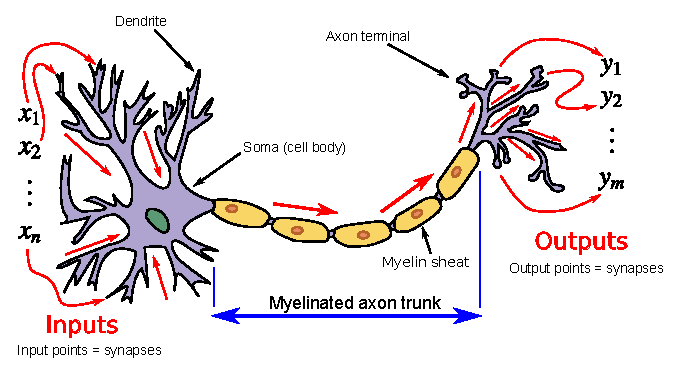
\includegraphics[width=0.7\textwidth]{figures/Neuron3.eps}
    \caption{neuron from \cite{wikipedianeuron}}
    \label{fig:neuron}
\end{figure}
Figure \ref{fig:neuron} shows a biological neuron with input and output synapses. Each 
of the input and output synapses is connected to other cells forming the neural 
network with billions of individual cells.
Without diving into the biochemical details, we can say that information is carried down the 
axon in the form of spike-like electric pulses, and transmitted through the synapse with 
the help of ions neurotransmitters and positive ions.
The electrical potential in the cells is typically $-70$mV. When a synapse receives a
signal, this potential slightly increases, and when it reaches a treshold of $\approx -55$mV, 
the cell fires, and a signal will be sent to the output synapses. 
Different input synapses have different importance, and thus they contribute to the 
output signal with different coefficients. Therefore, we can say that the output 
frequency of the $i$-th neuron is modeled by
\begin{equation}
    y_i = \theta\left(\sum\limits_j J_{ij}x_j - U_0\right),
\end{equation} 
where $\theta(x)$ is the Heaviside-step function, $x_j$ are input frequencies and $U_0=-55$mV is
the treshold potential.
From this model, we can derive a more general neuron model, which will be used to train 
deep neural networks:
\begin{equation}
    \mathbf y = g\left(\mathbf W^\top\mathbf x + \mathbf b\right),
\end{equation}
where $g$ is called \textit{activation function}, $\mathbf W$ and $\mathbf b$ are the 
\textit{weights} and \textit{bias}es, respectively.
Some commonly used activation functions are shown on figure \ref{fig:activations}. This model of a single neuron is called a 
perceptron. 
The simplest form of deep neural network uses many perceptrons and is called a \textit{multilayer-perceptron}
(MLP), see figure \ref{fig:MLP}. In this case the input vectors are fed into many perceptrons, and the 
outputs of these is fed into the perceptrons of the next layer. This architecture is often called 
fully connected or dense neural network, and the layers of perceptrons are called hidden layers. 
The outputs of an MLP can be scalars vector, or in some cases tensors of higher rank.
\begin{figure}[H]
    \centering
    \includegraphics[width=0.7\textwidth]{figures/MLP.pdf}
    \caption{The multilayer perceptron architecture. Green circles are the input features which 
    can be scalar or vector values, the yellow circles represent the weights and biases of the 
    perceptrons of the hidden layers, while the red circle is the output. Data flow is noted with 
    black arrows.}
    \label{fig:MLP}
\end{figure}
\begin{figure}[H]
    \centering
    \includegraphics[width=0.99\textwidth]{figures/activation_functions.pdf}
    \caption{The three most frequently used activation functions in deep neural networks.
    Left: the sigmoid function, middle: rectified linear unit (ReLU), right: leaky ReLU.}
    \label{fig:activations}
\end{figure}


There are many more sophisticated neural network architectures like convolutional neural networks (CNNs)
\cite{LeCun-CNN}, which are useful for image processing tasks, recurrent neural networks 
with internal long term memory \cite{SchmidhuberLSTM} for speech recognition or time-series 
forecasting, or transformers \cite{Transformer} for machine translation. 
To dive into the details of these complex deep neural network architectures is out of the 
scope of this thesis. 
We will, however explain the gradient descent (GD) algorithm, which makes it possible to train 
complex neural networks with the help of automatic differentiation.
The training of deep neural networks for various machine learning task
became possible after the proposal of backpropagation algorithm in 1986 by 
Geoffrey Hinton et. al. \cite{BackpropPaper}.
Essentially, training neural networks is finding the best weights $(\mathbf W^*, \mathbf b^*)\equiv
\pmb\theta^*$, for which a defined loss function $\mathcal L$ has minimum:
\begin{equation}
    \pmb\theta^* = \underset{\pmb\theta}{\arg\min}\,\mathcal L (\mathbf y, f(\mathbf x; \pmb\theta)),
\end{equation}
where $f(\cdot; \pmb\theta)$ represents the neural network. The idea of gradient descent is 
to find $\pmb\theta^*$ by starting at a random point $\pmb\theta^{(0)}$ and at each timestep
update theta in the direction of gradient. In the standard version of gradient-descent, 
we calculate the average loss $L = \frac{1}{N}\sum\limits_{k=1}^N \mathcal L(\mathbf y_k, f(\mathbf x_k; \pmb\theta^{(t)}))$
for the entire dataset to do a single step of gradient descent (see algorithm \ref{algo:gd}).
\begin{algorithm}[H]
    \caption{Gradient Descent}
    \begin{algorithmic}[1]
    \Procedure {GradientDescent}{$ \{(\mathbf x_k, \mathbf y_k)\}_{k=1}^N,\, f,\, \pmb\theta^{(0)},\, \mathcal L,\, \alpha^{(0)},\,  T$}
        \ForAll {$t \in \{0,...,T\}$}
            \State Calculate $L = \frac{1}{N}\sum\limits_{k=1}^N \mathcal L(\mathbf y_k, f(\mathbf x_k; \pmb\theta^{(t)}))$ 
            \ForAll{$\theta_j \in \pmb\theta$}
                \State Calculate the gradients $ \left. \frac{\partial L}{\partial \theta_j} \right|_{\theta_j = \theta_j^{(t)}}$
                \State Update the parameter $\theta_j^{(t+1)} \leftarrow \theta_j^{(t)} - \alpha_j^{(t)} \left. \frac{\partial L}{\partial \theta_j} \right|_{\theta_j = \theta_j^{(t)}}$
            \EndFor
        \EndFor
    \EndProcedure
    \end{algorithmic}
    \label{algo:gd}
\end{algorithm}

In many cases, the dataset is very large, and it turned out to be useful to split the dataset 
into mini-batches of a small size and calculate the losses and gradients for each individual 
min-batch. This version of gradient descent is called mini-batch stochastic gradient descent or 
mini-batch SGD, sometimes simply SGD. Using SGD instead of GD not only improves the overall perform
ance of the models, but usually reduces time needed for convergence.
In algorithm \ref{algo:gd}, $\alpha_j^{(t)}$ are called learning rates, which determine the 
magnitude of the gradient step. We used this notation because most modern GD algorithms like 
Adam \cite{Kingma2015AdamAM} use different learning rates for each parameter, and the 
value of learning rates is updated after each iteration. Initially, the learning rates are 
typically in the range $[10^{-4},10^{-1}]$.
Since the loss function $\mathcal L$ is in most cases not a globally convex hyperplane, it is 
very hard to find its global minimum by GD. In fact, it is not even possible to tell if the 
optimum found by a deep neural network is a global or local optimum. Therefore it is possible
for a network to get stuck in a local minimum, which is suboptimal. There are two solutions to 
this problem: one can run the same model parallely with different initial parameters $\pmb\theta^{(0)}$,
or we can use a cyclic learning rate. Using a cyclic learning rate means, that when the 
variance of $\mathcal L$ reaches close to zero, we increase the learning rate, so we try to 
push the model out of the minimum, in the hope that it will find a better solution.
\nd{write about overfitting}\\
\nd{write about softmax}
\begin{equation}
    \texttt{Softmax}:\mathbb R^m \rightarrow \mathbb R^m,~\left[\texttt{Softmax}(\mathbf x)\right]_j = \frac{e^{x_j}}{\sum\limits_ke^{x_k}}
    \label{eq:softmax}
\end{equation}

\section{Quantum Machine Learning}
QSVM paper = \cite{QSVMPaper}
HHL paper = \cite{HHLPaper}
Feature Hilbert Spaces = \cite{FeatureHilbertSpaces}
Quantum Hopfield Networks = \cite{QuantumHopfield}

\nd{related papers: quantum svm, Kernel methods, HHL algorithm for matrix inversion, quantum-inspired classical algos\\
motivation: summary from Lloyd paper, regression, classification, hybrid traning, encoding, inference\\
General structure: encoding, rotations and beamsplitter = interferometer, squeezing, interferometer, displacement, all = affine transformation + at the end non-linear, e.g., cubic phase operation (numeric instability switch to Kerr gates --> write at the performance test)  \\
Loss functions: regression, classification\\
Regularization: keep trace close to zero, non-Gaussian\\
}
\begin{figure}[H]
    \centering
    \includegraphics[width=0.6\textwidth]{figures/VQC-optimization.png}
    \caption{VQC-optimization.}
    \label{fig:VQC-optimization}
\end{figure}
\subsection{Variational Quantum Eigensolver}
\label{sec:vqe}
Variational Quantum Eigensolvers \cite{Peruzzo2014} are hybrid quantum-classical algorithms 
designed to find the lowest energy eigenvalue of some Hamiltonian $H$. VQEs are one 
of the most studied quantum algorithms because of their expected use cases in 
quantum chemistry and materials science 
\cite{Wei2020-QCHEM,VQE-HARTREE-FOCK,Kandala2017-VQE-QCHEM,PhysRevX-VQE-QCHEM}.
VQEs are a special class of variational quantum circuits, where the operator being 
measured is the Hamiltonian of some system.
The basic idea behind the variational quantum eigensolver is as follows. 
First we fix the structure of a parametric quantum circuit called the ansatz, defined by a 
unitary $U(\pmb\theta)$, where $\pmb\theta\in\mathbb{R}^m$ are real parameters. 
Then we start by some initial state $\ket{\psi_0}$, which is usually $\ket 0^{\otimes M}$ 
in the qubit setting. For the continuous variable setting, the initial state can be the vacuum state,
a displaced state, a squeezed state, or a photon number eigenstate.
After preparing the circuit, we evaluate the expectation value of the Hamiltonian
which is eventually the cost, or loss:
\begin{equation}
    \mathcal L(\pmb\theta) = \langle H \rangle = \bra{\psi_0}U^{\dagger}(\pmb\theta)HU(\pmb\theta)\ket{\psi_0}
\end{equation}
The goal is to minimize the loss $\mathcal L$ by iteratively updating the parameters $\pmb\theta$ with some update rule. This update rule can be any gradient-free \cite{Zhu2019} or gradient-based method \nd{idezet}. To use gradient descent optimization in the VQE setting, we need to evaluate the gradient
$\nabla_{\pmb\theta}\mathcal L$, which can be challenging, and is described in details in chapter \ref{sec:qgrad}. Algorithm \ref{algo:vqe} describes 
the variational quantum eigensolver with a general gradient-based learning method. Notice that we wrote $\alpha_j^{(t)}$ for the learning rate, since in most modern optimizers like Adam \cite{Kingma2015AdamAM}, each parameter has its own learning rate and it may depend on the number of iterations already done.
\begin{algorithm}[H]
    \caption{K-shot VQE}
    \begin{algorithmic}[1]
    \Procedure {K-VQE}{$H,K,T,\alpha$}
        \ForAll {$t \in \{1,...,T\}$}
            \State Prepare the ansatz $U(\pmb\theta)$
            \State Estimate the loss $\mathcal L = \bra{\psi_0}U^{\dagger}(\pmb\theta)HU(\pmb\theta)\ket{\psi_0}$ by averaging $K$ shots
            \ForAll{$\theta_j \in \pmb\theta$}
                \State Calculate the quantum gradient $\partial_{\theta_j}\mathcal L$
                \State Update the parameter $\theta_j \leftarrow \theta_j - \alpha_j^{(t)}\partial_{\theta_j}\mathcal L$
            \EndFor
        \EndFor
    \EndProcedure
    \end{algorithmic}
    \label{algo:vqe}
\end{algorithm}
\subsection{Quantum Neural Networks}
\label{sec:qnn}
Cv-Qnns -LLoyd = \cite{CVQNNLLoyd}
\subsection{Calculating the gradients of the parameters}
\label{sec:qgrad}
In this section, we introduce the theory of calculating quantum gradients in the continuous variable setting. 
We follow the notation of Shuld et. al. \cite{AnalyticGradientsSchuld}. A variational quantum circuit is 
defined by a unitary $U(\pmb\theta),\, \pmb\theta\in\mathbb{R}^m$, an initial state $\ket{\psi_0}$ and a measurment 
operator $B$. We can understand a variational citcuit as $f:\mathbb{R}^m \rightarrow \mathbb{R}$, \nd{The Schuld paper writes $f:\mathbb{R}^m \rightarrow \mathbb{R}^{\red n}$, maybe a typo???} 
which maps the circuit parameters to the expectation value of operator $B$:
\begin{equation}
    f(\pmb\theta) = \bra{\psi_0}U^{\dagger}(\pmb\theta) B U(\pmb\theta)\ket{\psi_0}   
\end{equation}
In gradient-based optimizations, we need the gradient $\nabla_{\pmb\theta} f$, and this eventually means calculating the partial derivatives
$\partial_{\mu}f,\,\mu\in\pmb\theta$. In the continuous variable setting, observables are usually polynomials of the quadrature operators $X_j$ and $P_j$.



\section{Results}
In this chapter we present the results of our numerical experiments. In section 
\ref{sec:regression-results} we present the results obtained by applying a CV QNN to some 
regression tasks, in section \ref{sec:classification-results} we discuss the performance of 
the QNN-s on various classification examples. Finally, in section \ref{sec:bh-vqe-results}
we present the performance of a continuous-variable VQE on finding the ground-state energy 
of a Bose-Hubbard model. These numerical experiments were run using 
Strawerry Fields \cite{Killoran2019strawberryfields, ApplicationsOfStrawberryFields}, an 
open-source software for simulating photonic quantum circuits an Tensorflow \cite{abadi2016tensorflow},
Google's open-source framework for calculating gradients via automatic differentiation. Although
these software packages are very powerful and efficient for computing matrix algebra and 
simulating quantum circuits, due to the exponential scaling of the Hilbert-space of CV quantum 
systems, we can not efficiently simulate quantum circuits with more then a few qumodes. Therefore, 
in the regression and classification example we use only two qumodes with cutoff dimension $10$,
while in the VQE setting we used four qumodes with cutoff dimension $5$.


\subsection{Classification}
\label{sec:classification-results}
In this section we present the architecture we used to solve different classification tasks
using quantum neural networks and of course we present the results as well. We tested 
the same ansatz circuit with the same loss function on three different synthetic datasets:
blobs, moons and circles (see figure \ref{fig:classification_results} a-c).
The datasets are generared with scikit-learn \cite{scikit-learn}, a python package which 
contains a lot of implementations of data preprocessing and machine learning algorithms. 
We use an Ansatz circuit architecture inspired by \cite{CVQNNLLoyd}, composed of beamsplitters, 
displacment and squeezing gates and Kerr nonlinearities. Figure \ref{fig:single_layer_classification}
shows the ansatz circuit with a single layer.

\begin{figure}[H]
    \centering
    \includegraphics[width=0.75\textwidth]{figures/Classifier-Circles-Ansatz.pdf}
    \caption{Ansatz circuit used in the classification task with the first layer.}
    \label{fig:single_layer_classification}
\end{figure}

In all three datasests we used, the feature vectors are two-dimensional spacial coordinates
$\mathbf x = (x_1,x_2)$, and we use displacement encoding to encode these vectors into quantum states.
We use three-mode quantum neural network, and therefore the encoding function is 
\begin{equation}
    (x_1, x_2) \mapsto \op D_1(x_1)\otimes\op D_2(x_2)\otimes I_3 \ket{0,0,0},
\end{equation}
and we can write $\op U(\mathbf x; \pmb\theta)$ as a product:
\begin{equation}
    \op U(\mathbf x; \pmb\theta) = \op U'(\pmb\theta)\left(\op D_1(x_1)\otimes\op D_2(x_2)\otimes I_3\right).
\end{equation}
To construct the loss function, we use homodyne measurements with \texttt{Softmax} and \texttt{CrossEntropy}.
Depending on the number of classes in the dataset we measure modes $1-3$ in the case of blobs
or $2-3$ in the case of moons and circles.
The loss is simply
\begin{equation}
    \mathcal L =  \texttt{CrossEntropy}(\mathbf y^{\textrm{pred}}, \mathbf y^{\textrm{true}}) + \frac{\lambda}{|\mathcal B|}\sum||W^{\textrm{active}}||^2,
\end{equation}
where
\begin{equation}
    \mathbf y^{\textrm{pred}} = \texttt{Softmax}\begin{bmatrix}
        \textrm{abs}\left(\Tr{\op\rho \op X_1}\right) \\[6.5pt]
        \textrm{abs}\left(\Tr{\op\rho \op X_2}\right) \\[6.5pt]
        \textrm{abs}\left(\Tr{\op\rho \op X_3}\right) \\[6.5pt]
    \end{bmatrix}~\textrm{or}~
    \mathbf y^{\textrm{pred}} = \texttt{Softmax}\begin{bmatrix}
        \textrm{abs}\left(\Tr{\op\rho \op X_2}\right) \\[6.5pt]
        \textrm{abs}\left(\Tr{\op\rho \op X_3}\right) \\[6.5pt]
    \end{bmatrix},
\end{equation}
and $W^{\textrm{active}}$ are the weigths of the active gates in the QNN. 
This way, assuming that the output state of the QNN is pure, we can write
\begin{equation}
    \rho = \ketbra{\psi}{\psi}\, \textrm{with}\, \ket\psi = \op U(\mathbf x; \pmb\theta)\ket{\psi_0}.
\end{equation}
In most cases this assumption is true in our simulations, because we use $L^2$ normalization
on the active weights of the network, and thus $\Tr{\rho^2}\approx 1$.

\newcommand{\thisfigurewidth}{0.31}
\begin{figure}[H]
    \centering
    \begin{tabular}{ccc}
      \includegraphics[width=\thisfigurewidth\textwidth]{figures/fig_dataset_blobs.png} & 
      \includegraphics[width=\thisfigurewidth\textwidth]{figures/fig_dataset_circles.png} &
      \includegraphics[width=\thisfigurewidth\textwidth]{figures/fig_dataset_moons.png} \\
      (a) & (b) & (c) \\[6.5pt]
      \includegraphics[width=\thisfigurewidth\textwidth]{figures/test_acc_blobs_lr=0_1.png} & 
      \includegraphics[width=\thisfigurewidth\textwidth]{figures/test_acc_circles_lr=0_1.png} &
      \includegraphics[width=\thisfigurewidth\textwidth]{figures/test_acc_moons_lr=0_001.png} \\
      (d) & (e) & (f) \\[6.5pt]
      \includegraphics[width=\thisfigurewidth\textwidth]{figures/test_loss_blobs_lr=0_001.png} & 
      \includegraphics[width=\thisfigurewidth\textwidth]{figures/test_loss_circles_lr=0_1.png} &
      \includegraphics[width=\thisfigurewidth\textwidth]{figures/test_loss_moons_lr=0_001.png} \\
      (g) & (h) & (i) \\[6.5pt]
    \end{tabular}
    \caption{leiras}
    \label{fig:classification_results}
\end{figure}

\begin{figure}[H]
    \centering
    \includegraphics[width=0.5\textwidth]{figures/classifier-test-acc-shots.png}
    \caption{}
    \label{fig:single_layer_regression}
\end{figure}


\subsection{Regression}
\label{sec:regression-results}
As specified earlier, the aim of regression is to predict or forecast a value $y$ for 
previously unseen feature vectors $\mathbf x$ by inferring a function $f$ from 
given example pairs $(\mathbf x_k, y_k)$. 
In this chapter, we present our results on testing regression with parametric quantum 
circuits on a photonic CV architecture.
We test our methods on synthetic datasets, as well as on a real-world dataset.
In the simulations presented hereby, both the feature and the dependent
value are scalars. 
\nd{Data normalization and encoding}
Data normalization is usually 
a very important step in order to achieve good performance in machine learning.
Therefore, we normalized our datasets so
that most of the $x$ and $y$ values fall into the $[-1,1]$ interval.
In chapter \ref{sec:qnn} we saw that encoding classical data into a quantum state is a 
crucial step in quantum machine learning. Therefore we tested different encodings 
and found that displacement encoding works the best in each of the simulations.
Hence, in all of the simulations presented in this thesis we use displacement encoding, which means that 
the feature $x$ is encoded into the quantum system by applying a single-mode Weyl-displacement
operator $\op D(x)$ on one or more modes. In the regression task, we apply the same displacement
on all of the modes:
\begin{equation}
    x \mapsto \op D_1(x)\otimes\op D_2(x) \ket{0,0}.
\end{equation}
This way the unitary matrix in equation \ref{eq:regression-output} can be written as 
\begin{equation}
    \op U(x;\pmb\theta) = \op U'(\pmb\theta) \left(\op D_1(x)\otimes\op D_2(x)\right),
\end{equation}
where $\op U'(\pmb\theta)$ does not depend on the value of $x$.
After data encoding, we apply a number of identical quantum layers composed of beamsplitters, 
rotations, displacements, squeezing gates and Kerr nonlinearities. These gates are arranged in 
a structure similar to that prosed in \cite{CVQNNLLoyd}.
\nd{Weight normalization}
Another important step to consider is weight normalization. Since passive photonic gates 
do not change the overall energy of the system, we do not apply any kind of normalization 
to the parameters of the passive gates. Active gates however like displacement and squeezing
change the energy of the system (or photon number), and thus they can push the state 
into a mixed state \cite{CVQNNLLoyd}, which we want to avoid as much as possible.
Therefore we apply an $L^2$-regularization to the active weights $W^{\textrm{active}}$ of the 
network. Therefore the loss function we use in the regression test is
\begin{equation}
    \mathcal L = \frac{1}{|\mathcal B|}\sum\limits_{(x,y)\in\mathcal B} \left(y - \Tr{\op\rho \op X_2} \right)^2 + \frac{\lambda}{|\mathcal B|}\sum||W^{\textrm{active}}||^2.
\end{equation}
where $\mathcal B$ is a mini-batch of size $|\mathcal B|$ and $\op \rho$ is the otput of the quantum neural network.
Some regression tasks work better if we use $L^1$ regularization, or even both $L^1$ and $L^2$,
but we found that $L^2$ regularization works perfectly fine in our cases.
Assuming that the output state is pure, we can write
\begin{equation}
    \op \rho = \ketbra{\psi}{\psi},\, \textrm{with}\, \ket\psi = \op U(x;\pmb\theta)\ket{\psi_0}.
    \label{eq:regression-output}
\end{equation}


We tested the performance of the QNN with different number of layers (see figure \ref{fig:tanh_layer_search}), 
and concluded that we need at least six layers to achieve the target MSE of $0.002$ on the test set.
The quantum neural network we use in the regression task is shown on figure \ref{fig:BasicTwoModeRegressor}.

\begin{figure}[H]
    \centering
    \includegraphics[width=0.75\textwidth]{figures/BasicTwoModeRegressor-circuit.pdf}
    \caption{Ansatz circuit for the regression task. We use displacement encoding and 
    six consecutive identical layers with a homodyne measurement at the end.}
    \label{fig:BasicTwoModeRegressor}
\end{figure}

\begin{figure}[H]
    \centering
    \includegraphics[width=0.5\textwidth]{figures/tanh-test-mse-lr=0_001-bs=150-layersearch.pdf}
    \caption{Comparison of the regression circuit performance on the test set
    with different number of layers.}
    \label{fig:tanh_layer_search}
\end{figure}

We tested the quantum neural network described above on two \nd{three?} datasets: one of them was a
synthetic dataset, namely the $f(x)=\tanh(\pi x)$ function \nd{$x^3$?} the other one is a normalized
I-V curve of a photodiode.
We run a bunch of numerical experiments experiments

\begin{table}[H]
    \centering
    \begin{tabular}{|c|c|c| } 
     \hline
     &  $\tanh$ & I-V \\ \hline
     \#training data & $105$ & $100$\\ \hline 
     \#test data & $45$ & $38$\\ \hline 
     \#layers & $6 $& $6$ \\ \hline
     \#qumodes & $2$ & $2$ \\ \hline
     \#shots & $50$ to $1000$ & $50$ to $1000$ \\ \hline
     mini-batch size & $4$ & $4$ \\ \hline
     $\lambda$ & $0.1$ & $0.1$ \\ \hline
     lr & $0.001$ & $0.001$ \\ \hline
     \hline
    
    \end{tabular}
    \caption{Hyperparameters of the regression simulations}
    \label{tab:hyperparams-regression}
\end{table}

\renewcommand{\thisfigurewidth}{0.33}
\begin{figure}[H]
    \centering
    \begin{tabular}{ccc}
      \includegraphics[width=\thisfigurewidth\textwidth]{figures/tanh-test-mse-bs=4-lr=0_001-shotsearch.pdf} & 
      \includegraphics[width=\thisfigurewidth\textwidth]{figures/iv-test-mse-bs=4-lr=0_001-shotsearch.pdf} &
      \includegraphics[width=\thisfigurewidth\textwidth]{figures/x2-test-mse-bs=4-lr=0_001-shotsearch.pdf} \\
      (a) & (b) & (c) \\[6.5pt]
      \includegraphics[width=\thisfigurewidth\textwidth]{figures/tanh-results-bs=16-lr=0_001-s1000.pdf} & 
      \includegraphics[width=\thisfigurewidth\textwidth]{figures/iv-bs=4-lr=0_001-s1000.pdf} &
      \includegraphics[width=\thisfigurewidth\textwidth]{figures/x2-bs=4-lr=0_001-s1000.pdf} \\
      (d) & (e) & (f) \\[6.5pt]
    \end{tabular}
    \caption{The top row shows how the regression circuits perform on the test set. The figures show
    loss curves with different number of shots for the $\tanh$ function (a) and the I-V curve (b).
    The bottom rows show inference tests with $1000$ shots both for the $\tanh$ function (c) as well
    as the I-V curve (d).
    All simulations were run with $\alpha=0.001$ and mini-batch size $4$.\\
    \nd{Change tanh-results-bs=16-lr=0\_001-s1000.pdf to tanh-results-bs=\red{4}-lr=0\_001-s1000.pdf}\\
    \nd{increase tick size on inference plots}
    }
    \label{fig:regression_results}
\end{figure}

\subsection{CV-VQE for the Bose-Hubbard model}
\label{sec:bh-vqe-results}
The Bose-Hubbard model introduced first by Gersch and Knollman in 1963 for the description of interacting spinless bosons on a lattice, such as ultracold bosonic atoms on an optical lattice
\cite{BoseHubbardOriginal,ColdAtomtHubbard}. This model has also gained popularity because it is found to be an adequate model for the description of the Superfluidity-Mott insulator (SF-MI) transition, which has been experimentally demonstrated \cite{SuperfluidityMottTransition,Greiner2002}.
We chose this model, because an exact diagonalization of the Bose-Hubbard Hamiltonian with respect to a finite dimensional Fock-basis is possible and thus the model is numerically solvable. This enables the verification of the correctness of the results given by our variational quantum solver for small problem instances.
\par
The Bose Hubbard model which we used in our simulations is defined by the following Hamiltonian expressed with the bosonic creation and annihillation operators:
\begin{equation}
     H = -t\sum\limits_{i=1}^{M-1}( a_{i}^\dagger  a_{i+1} +  a_{i+1}^\dagger  a_{i}) + \frac{U}{2}\sum\limits_{i=1}^{M} n_i^2 ,
     \label{eq:bhhamiltonian}
\end{equation}
where $M$ is the number of bosonic modes in the system. If we restrict the total number of bosons in the system to be $N$, the dimension of the restricted Fock-space is
\begin{equation}
    D = \frac{(N+M-1)!}{N!(M-1)!},
\end{equation}
which explosively grows with the system size. Therefore finding the groundstate of the Bose-Hubbard Hamiltonian for larger systems can be intractable even on classical supercomputers, making quantum computers, especially continuous-variable quantum computers a potential candidate for solving these problems in the future.
Compared to the original definition of the Bose-Hubbard Hamiltonian, we omitted the term $-\mu\sum\limits_{i}^{M} n_i$, because it is not relevant in our particular experiments.


\subsubsection{Solving the model by exact diagonalization}
\nd{Analytic solution by diagonalization}
If we want to calculate the groundstate of a Bose-Hubbard model, then we need to solve the 
eigenvalue-problem of Hamiltonian \ref{eq:bhhamiltonian}.
Of course a general Fock-space corresponding to a bosonic system is infinite-dimensional, therefore
we have to restrict the system so that a maximum of $N$ particles are allowed in each mode:
\begin{align*}
|0,0, ..., 0\rangle, |0,0, ..., N\rangle, |0,0, ..., 1, N\rangle, ... |N,N,...,N\rangle.
\end{align*}
Then, we can relabel the Fock-states so that each Fock basis has its own unique label $j$:
\begin{equation}
|n_{M-1}, n_{M-2}, ... n_{1}, n_{0}\rangle = \left|\sum\limits_{k=0}^{M-1}n_{k}(N+1)^{k}\right\rangle.
\end{equation}
This is useful, because with these relabeled states we can calculate the matrix elements of the new 
Hamiltonian:
\begin{equation}
    H_{jj'} = \bra{j}H\ket{j'} = \langle n_{M-1}, n_{M-2}, ... n_{1}, n_{0}| H |n'_{M-1}, n'_{M-2}, ... n'_{1}, n'_{0}\rangle
\end{equation}
We can further reduce the dimension of the Hilbert space if we prescribe that the total number of photons
must be $N$:
\begin{equation*}
    \sum\limits_kn_k = N.
\end{equation*}
In this case for example if the number of modes is $M=4$ and the total number of particles is $N=4$,
the dimension of the restricted Hilbert-space is only $35$.

The resulting matrix $H_{jj'}$ is usually a sparse matrix (see fig. \ref{fig:exactdiagonalization}),
and can be diagonalized using existing software.
\begin{figure}[H]
    \centering
    \begin{tabular}{cc}
      \includegraphics[height=0.2\textheight]{figures/real_fock_matrix_M=4_cutoff=4_t=-0_5_U=-0_5.pdf} & \includegraphics[height=0.2\textheight]{figures/diagonalized_solutions_M=4_cutoff=4.pdf} \\
      (a) & (b) \\[6pt]
    \end{tabular}
    \caption{(a) Visual representation of a sparse Hamiltonian matrix $H_{jj'}$ for a Bose-Hubbard model
    with $\dim(\mathcal H)=35$.
    Darker points show the non-zero elements in the matrix (b) Numerical solutions of the ground-state
    energy for different $U$ and $t$ values.}
    \label{fig:exactdiagonalization}
\end{figure}

\subsubsection{Variational solutions}
VQEs introduced in section \ref{sec:vqe} are shown to be effective for simulating
different fermionic quantum systems, like molecules or metals 
\cite{Wei2020-QCHEM, VQE-HARTREE-FOCK, Kandala2017-VQE-QCHEM, PhysRevX-VQE-QCHEM}.
In this chapter we demonstrate a photonic VQE for finding the ground-state energy of a Bose-Hubbard model.
Furthermore, we show that stochastic gradient descent methods can be applied to the VQE to reduce
the number of shots required, and thus reduce the overall cost of finding the ground state energy
on a quantum hardware.
\par
The variational circuit $U(\pmb\theta)$ can be realized with sequences of quantum gates, in our case
photonic quantum gates.
Since we want the total number of particles in the system to be preserved during the simulations,
we must use photon-number preserving gates only. We composed each quantum layer from 
Beamsplitters, Kerr-gates and Cross-Kerr-gates (see fig. \ref{fig:single_layer_vqe}).
\begin{figure}[H]
    \centering
    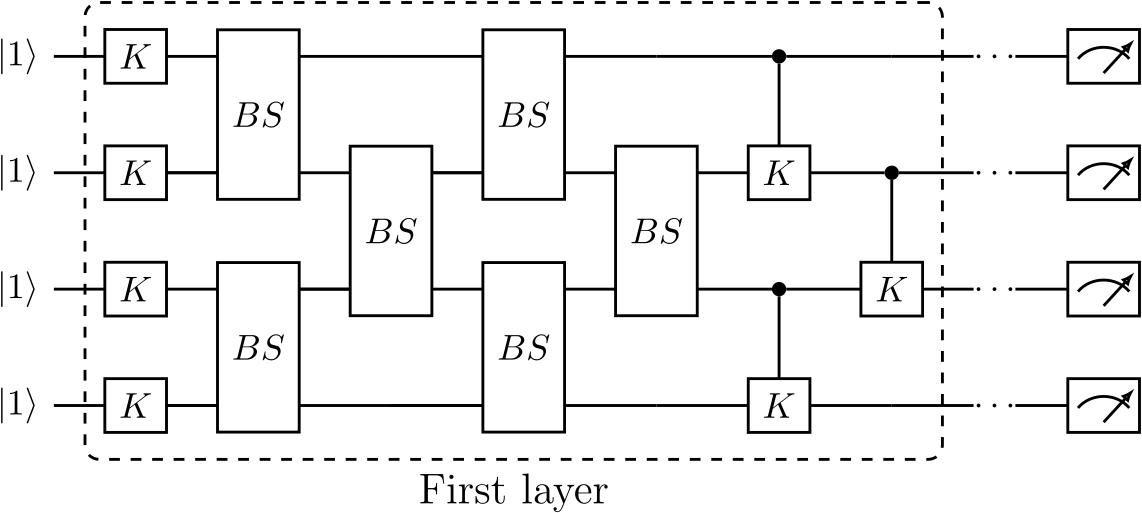
\includegraphics[width=0.66\textwidth]{figures/BH-Ansatz.pdf}
    \caption{Illustration of a variational ansatz circuit with its first layer. Initially, each of the four qumodes contain a
    single photon. The layer is built up from Kerr-gates, CrossKerr gates and Beamsplitters, which are passive optical gates, so the
    total number of photons is preserved.}
    \label{fig:single_layer_vqe}
\end{figure}
Throughout the numerical experiments, we set initially one single photon in each of the four qumodes i.e.
$\ket{\psi_0}=\ket{1}^{\otimes M}$, and applied a number of identical quantum layers 
followed by quadrature measurements.
\begin{figure}[H]
    \centering
    \includegraphics[width=0.66\textwidth]{figures/BH-layersearch-2.pdf}
    \caption{}
    \label{fig:single_layer_vqe}
\end{figure}

\begin{figure}[H]
    \centering
    \begin{tabular}{cc}
      \includegraphics[width=0.5\textwidth]{figures/BH-stoch-L=6-t=-0_5-U=-0_5-lr=0_001-shots=5-50.pdf} &   \includegraphics[width=0.5\textwidth]{figures/BH-stoch-L=6-t=-0_5-U=-0_5-lr=0_001-shots=100-5000.pdf} \\
    (a) first & (b) second \\[6pt]
     \includegraphics[width=0.5\textwidth]{figures/BH-doublystoch-bs=12-L=6-t=-0_5-U=-0_5-lr=0_001-shots=5-50.pdf} &   \includegraphics[width=0.5\textwidth]{figures/BH-doublystoch-bs=12-L=6-t=-0_5-U=-0_5-lr=0_001-shots=100-5000.pdf} \\
    (c) third & (d) fourth \\[6pt]
    \end{tabular}
    \caption{caption}
\end{figure}

\section{Conclusion and future work}

\bibliography{references}
%%%%%%%%%%%%%%%%%%%%%%%%%%%%%%%%%%%%%%%%%%%%%%%%%%%%%%%%%%%%%%%%%%%%%%%%%%%%%%%%%%%%%%%%%%%%%%%%%%%
%%%%%%%%%%%%%%%%%%%%%%%%%%%%%%%%%%%%%%%%%%%%%%%%%%%%%%%%%%%%%%%%%%%%%%%%%%%%%%%%%%%%%%%%%%%%%%%%%%%
%
%                    APPENDIX
%
%%%%%%%%%%%%%%%%%%%%%%%%%%%%%%%%%%%%%%%%%%%%%%%%%%%%%%%%%%%%%%%%%%%%%%%%%%%%%%%%%%%%%%%%%%%%%%%%%%%
%%%%%%%%%%%%%%%%%%%%%%%%%%%%%%%%%%%%%%%%%%%%%%%%%%%%%%%%%%%%%%%%%%%%%%%%%%%%%%%%%%%%%%%%%%%%%%%%%%%


\appendix
\section{Coherent states}
\label{appendix:coherent}
A coherent state is the eigenstate of $\hat a$:
\begin{equation*}
    \hat a \ket{\alpha} = \alpha\ket{\alpha}
\end{equation*}
\begin{align*}
    \ket\alpha = \sum\limits_{n=0}^{\infty}\ket n\braket{n|\alpha}
\end{align*}
we have
\begin{align*}
    &\hat a\ket\alpha = \alpha\ket\alpha \implies \braket{n|\hat a|\alpha}=\alpha\braket{n|\alpha}
\end{align*}
and 
\begin{align*}
    &\hat a^{\dagger}\ket n = \sqrt{n+1}\ket{n+1} \implies \bra n \hat a = \sqrt{n+1}\bra{n+1}\\
    &\implies \braket{n|\hat a|\alpha} = \sqrt{n+1}\braket{n+1|\alpha} = \alpha\braket{n|\alpha}\\
    &\implies \braket{n|\alpha} = \frac{\alpha}{\sqrt n}\braket{n-1|\alpha} = \dots = \frac{\alpha^n}{\sqrt{n!}}
    \braket{0|\alpha}
\end{align*}
therefore,
\begin{align*}
    \ket\alpha = \sum\limits_{n=0}^{\infty}\frac{\alpha^n}{\sqrt{n!}}\braket{0|\alpha}\ket n
\end{align*},
The value of $\braket{0|\alpha}$ can be calculated from the normalization condition
$\braket{\alpha|\alpha}\overset{!}{=}1$. Since
\begin{align*}
    &\ket\alpha = \braket{0|\alpha}\sum\limits_{n=0}^{\infty}\frac{\alpha^n}{\sqrt{n!}}\ket n \\ 
    &\bra\alpha = \braket{\alpha|0}\sum\limits_{k=0}^{\infty}\frac{(\alpha^*)^k}{\sqrt{k!}}\bra k,
\end{align*}
we have 
\begin{align*}
    1\overset{!}{=} \braket{\alpha|\alpha} & = 
    \left(\braket{\alpha|0}\sum\limits_{k=0}^{\infty}\frac{(\alpha^*)^k}{\sqrt{k!}}\bra k\right)
    \left(\braket{0|\alpha}\sum\limits_{n=0}^{\infty}\frac{\alpha^n}{\sqrt{n!}}\ket n\right)\\
    &=\braket{\alpha|0}\braket{0|\alpha}\sum\limits_{k=0}^{\infty} \sum\limits_{n=0}^{\infty}
    \frac{(\alpha^*)^k\alpha^n}{\sqrt{k!n!}}\braket{k|n} \\
    &=\braket{\alpha|0}\braket{0|\alpha}\sum\limits_{k=0}^{\infty} \sum\limits_{n=0}^{\infty}
    \frac{(\alpha^*)^k\alpha^n}{\sqrt{k!n!}}\delta_{kn}\\
    &= |\braket{0|\alpha}|^2 \sum\limits_{n=0}^{\infty} \frac{(|\alpha|^2)^n}{n!} = |\braket{0|\alpha}|^2e^{|\alpha|^2}.
\end{align*}
\begin{equation*}
    \implies \braket{0|\alpha} = e^{i\varphi}e^{-\frac{|\alpha|^2}{2}}
\end{equation*}
And so, a coherent state can be written as 
\begin{equation*}
    \ket\alpha = e^{i\varphi}e^{\frac{-|\alpha|^2}{2}}\sum\limits_{n=0}^{\infty}\frac{\alpha^n}{\sqrt{n!}}\ket n
\end{equation*}
\section{Mathematical preliminaries}
\label{appendix:mathematical-preliminaries}

\subsection{Hilbert spaces}
\label{appendix:Hilbertspace}
\begin{definition}
    \textbf{Hilbert-space}\\
    Given a field $T$ (real or complex), a vector space $\mathcal H$ endowed with an inner product, is called a Hilbert-space, if
    it is a complete metric space with respect to the distance function induced by the inner product.
    \\
    The inner product is a map $\braket{\cdot|\cdot}:\mathcal{H}\times\mathcal{H} \rightarrow T$, 
    for which $\forall x,y,z \in \mathcal H$:
    \begin{itemize}
        \item $\braket{x|x} \geq 0$
        \item $\braket{x|x} = 0 \Longleftrightarrow x = \bb 0 \in \mathcal H$
        \item $\braket{x|y} = \braket{y|x}^*$, where $^*$ denotes complex conjugation.
        \item $\braket{x|\alpha y + \beta z} = \alpha\braket{x|y} + \beta\braket{x|z}$, where $\alpha, \beta \in T$
    \end{itemize}
    The norm induced by this inner product is a map $||\cdot||:\mathcal H \rightarrow T$ defined as
    \begin{equation*}
        ||x||=\sqrt{\braket{x|x}},
    \end{equation*}
    And the metric induced by this norm is defined as
    \begin{equation*}
        d(x,y) = ||x - y|| = \sqrt{\braket{x - y|x - y}}.
    \end{equation*}
    The space $\mathcal H$ is said to be complete if every Cauchy-sequence is convergent with respect to the norm, and
    the limit is in $\mathcal H$. That is, each sequence ${x_1, x_2, ... }$, for which 
    \begin{equation*}
        \forall \varepsilon > 0 ~ \exists N(\varepsilon) ~\textrm{so, that}~ n>m>N(\varepsilon) \implies ||x_n - x_m||<\varepsilon.
    \end{equation*}
\end{definition} 

\begin{definition}
    \textbf{Linear functional}\\
    Let $\mathcal H$ be a Hilbert-space over the field $T$. Then, the map $\varphi:\mathcal H \rightarrow T$ is  
    called a linear functional, if
    \begin{equation*}
        \varphi(\alpha x + \beta y) = \alpha \varphi(x) + \beta \varphi(y),~
        \forall \alpha, \beta \in T,\, x, y \in \mathcal H.
    \end{equation*}
\end{definition}

\begin{definition}
    \textbf{Dual space}\\
    Given a Hilbert-space $\mathcal H$, its dual space, $\mathcal H^*$ is the space of all continuous linear
    functionals from the space H into the base field.
    The norm of an element in $\mathcal H^*$ is 
    \begin{equation*}
        ||\varphi||_{\mathcal H^*} \overset{def}{=} \underset{||x||=1,\, x \in \mathcal H}{\sup} |\varphi(x)|.
    \end{equation*}
\end{definition}

\begin{theorem}
    \textbf{Riesz representation theorem}\\
    For every element $y \in \mathcal H$, there exists a unique element $\varphi_{y} \in \mathcal H^*$, defined by
    \begin{equation*}
        \varphi_{y}(x) = \braket{y| x},~\forall x \in \mathcal H.
    \end{equation*}
    The mapping $y \mapsto \varphi_{y}$ is an antilinear mapping i.e. $\alpha y_1 + \beta y_2 
    \mapsto \alpha^* \varphi_{y_1} + \beta^* \varphi_{y_2}$, and the Riesz-representation theorem states 
    that this mapping is an antilinear isomorphism. The inner product in $\mathcal H^*$ satisfies 
    \begin{equation*}
        \braket{\varphi_{x}|\varphi_{y}} = \braket{x|y}^* = \braket{y | x}.
    \end{equation*}
    Moreover, $||y||_{\mathcal H} = ||\varphi_{y}||_{\mathcal H^*}$.
\end{theorem}

\begin{definition}
    \textbf{Dirac-notation}\\
    From now on, the elements in $\mathcal H$ will be denoted by $\ket x$ and their corresponding
    element in $\mathcal H^*$ as $\bra x$.
\end{definition}

\subsection{Linear operators on Hilbert spaces}
\label{appendix:linear-ops}
\begin{definition}
    \textbf{Linear operators}\\
    A map $\hat A: \mathcal H_1 \rightarrow \mathcal H_2$ is a linear operator, if 
    \begin{equation*}
        \hat A (\alpha\ket x + \beta\ket y) = \alpha (\hat A \ket x) + \beta (\hat A \ket y).
    \end{equation*}
\end{definition}

\begin{remark}
    If not stated otherwise, we will assume that $\mathcal H_1 = \mathcal H_2 = \mathcal H$.
\end{remark}

\begin{remark}
    Operators will be denoted with a hat ($\hat{\cdot}$).
\end{remark}

\begin{definition}
    \textbf{Bounded linear operators}\\
    A linear operator $\hat A: \mathcal H \rightarrow \mathcal H$ is bounded, if 
    \begin{equation*}
        \exists m \in \mathbb R : |\braket{v|\hat A | v}| \leq m\braket{v|v},\, \forall \ket v \in \mathcal H
    \end{equation*}
\end{definition}

\begin{remark}
    The set of all bounded operators on $\mathcal H$ is denoted $\mathcal{B(H)}$.
\end{remark}


\begin{definition}
    \textbf{Commutators and anticommutators}\\
    Since operators usually do not commute, its useful to define their commutator and anticommutator:
    \begin{align*}
        &[\hat A, \hat B] = \hat A\hat B - \hat B\hat A\\
        &\{\hat A, \hat B\} = \hat A\hat B + \hat B\hat A
    \end{align*}
\end{definition}

\begin{definition}
    \textbf{Operator norm}\\
    The operator norm of an operator $\hat A$ is defined as 
    \begin{equation*}
        ||\hat A|| \overset{def}{=} \inf\{c\geq 0 : ||\hat A\ket v || \leq c ||\ket v||,\,\forall \ket v \in \mathcal H \}
    \end{equation*}
\end{definition}

\begin{definition}
   \textbf{Trace-class operators}\\
   An operator $\hat A$ is called trace-class if it admits a well defined and finite trace 
   $\Tr{\hat A} = \sum\limits_j\braket{j|\hat A|j}$
\end{definition}

\begin{definition}
    \textbf{Positive operators}\\
    An operator $\hat A$ is called positive if $\braket{v|\hat A|v} \geq 0,\,\forall \ket v \in \mathcal{H}$.
    If $\hat A = \sum\limits_j \lambda_j \ket j \bra j$ then $\hat A$ is positive if $\lambda_j \geq 0$.
\end{definition}

\begin{definition}
    \textbf{Projections}
    An operator $\Pi:\mathcal H \rightarrow \mathcal H$ is a projection if $\Pi^2=\Pi$.
\end{definition}

\subsection{Hermitian Operators, Unitary Operators, Spectral theorem, Hadamard-lemma}
\begin{definition}
    \textbf{Hermitian adjoint}
    \\Consider a \textbf{bounded} linear operator $\hat A: \mathcal H \rightarrow \mathcal H$. The hermitian adjoint of 
    $\hat A$ is a bounded linear operator $\hat A^\dagger : \mathcal H \rightarrow \mathcal H$ which satisfies
    \begin{equation}
        \bra y \hat A \ket x = \left( \bra x \hat A^\dagger \ket y \right)^*, ~\forall \ket x, \ket y \in \mathcal H.
    \end{equation}
\end{definition}

\begin{definition}
    \textbf{Hermitian operators}
    \\ A bounded linear operator $\hat H : \mathcal H\rightarrow \mathcal H$ is Hermitian if 
    \begin{equation}
        \hat H = \hat H^\dagger, \textrm{ i.e. } \hat H\ket x = \hat H^\dagger \ket x, ~\forall \ket x \in \mathcal H.
    \end{equation}
\end{definition}

\begin{definition}
    \textbf{Unitary operator}
    \\A bounded linear operator $\hat U : \mathcal H\rightarrow \mathcal H$ is unitary if 
    \begin{equation}
        \hat U\hat U^\dagger = \hat U^\dagger \hat U = 1, \textrm{ in other words, } \hat U^{\dagger} = \hat U^{-1}. 
    \end{equation}
\end{definition}

\begin{definition}
    \textbf{Eigenvalues and eigenvectors}
    \\Consider bounded linear operator $\hat A$. If exist a vectors $\ket k \in \mathcal H$ such that
    \begin{equation}
        \hat A \ket k = \lambda_k\ket k,
    \end{equation}
    then $\ket k$ is called an eigenvector of $\hat A$ and $\lambda k$ is the corresponding eigenvalue.
\end{definition}

An important property of Hermitian operators is that they can be diagonalized with real eigenvalues. 
This is formally stated by the spectral theorem:
\begin{theorem}
    \textbf{The Spectral theorem}
    \\Let $\hat A$ be a bounded Hermitian operator on some Hilbert-space $\mathcal H$. Then there exists an orthonormal
    basis in $\mathcal H$ which consists of the eigenvectors of $\hat A$ and each eigenvalue of $\hat A$ is real.
\end{theorem}
This means that any bounded Hermitian operator $\hat H$ can be decomposed as 
\begin{equation}
    \hat H = \sum\limits_{k}\lambda_k \hat P_k = \sum\limits_{k}\lambda_k \ketbra{k}{k}
\end{equation}
where $\lambda_k$ and $\ket k$ are the eigenvalues and eigenvectors of $\hat H$.


\begin{definition}
    \textbf{Exponential of operators}
    If $X$ is a linear operator, we can define the exponential of $X$:
    \begin{equation*}
        e^X = \sum\limits_{n=0}^\infty \frac{X^n}{n!} 
    \end{equation*}
\end{definition}
\textbf{Important}:
The product of exponentials of operators generally isn't equal to the exponential of their sum:
\begin{equation*}
    e^{X}e^{Y} = e^{Z(X,Y)}\neq e^{X+Y},
\end{equation*}
where $Z(X,Y)$ is given by the Baker-Campbell-Hausdorff formula:
\begin{align*}
    Z(X,Y) &= X + Y + \frac{1}{2}[X,Y] + \frac{1}{12}[X,[X,Y]] - \frac{1}{12}[Y,[X,Y]] -\frac{1}{24}[Y,[X,[X,Y]]] \\
    & - \frac{1}{720}([[[[X,Y],Y],Y],Y] + [[[Y,X],X],X],X]) + ...
\end{align*}
It is however equal if $[X,Y]=0$:
\begin{equation*}
    \textrm{if}\,[X,Y]=0 \implies  e^{X}e^{Y} = e^{X+Y}
\end{equation*}
There are 2 important special cases:
\begin{theorem}
    \textbf{The Hadamard-lemma}
    \begin{equation*}
        e^XYe^{-X} = Y + [X,Y] + \frac{1}{2!}[X,[X,Y]] + \frac{1}{3!}[X,[X,[X,Y]]] + ...
    \end{equation*}
\end{theorem}

\begin{theorem}
    If $X$ and $Y$ commute with their commutator, i.e. $[X, [X,Y]] = [Y, [X,Y]] = 0$, then:
    \begin{equation*}
        e^Xe^Y = e^{X+Y+\frac{1}{2}[X,Y]}
    \end{equation*}
\end{theorem}

\begin{theorem}
    If $[X,Y] = sY$ with $s\in\mathbb{C}, s\neq 2i\pi n, n\in \mathbb Z$ then:
    \begin{equation*}
        e^Xe^Y = \exp\left(X + \frac{s}{1-e^{-s}}Y \right)
    \end{equation*}
\end{theorem}

\subsection{Pure and mixed quantum states}
\label{appendix:pure-and-mixed-states}
\begin{definition}
    \textbf{Quantum states}\\
    A quantum state of a quantum system is a mathematical entity that provides a probability distribution 
    for the outcomes of each possible measurement on the system.
\end{definition}

\begin{definition}
    \textbf{Pure quantum states}\\
    Pure quantum states are quantum states that can be described by a vector $\ket\psi$ of norm 1. 
\end{definition}
If one multiplies a pure quantum state by a complex scalar $e^{i\alpha}$, then the new state is 
physically equivalent to the former, thus $\ket\psi$ and $e^{i\alpha}\ket\psi$ are 
the same pure state.
The transformation $\ket\psi\rightarrow e^{i\alpha}\ket\psi$ does not change the outcomes of measurements on the state,
however the phase $\alpha$ is important in quantum algorithms.
\begin{example*}
    For example, the states $\frac{1}{\sqrt 2}(\ket 0 + e^{i\pi}\ket 1)$ and $\frac{1}{\sqrt 2}(\ket 0 + e^{i\frac{\pi}{2}}\ket 1)$
    are not the same quantum state, but in both states there is 50-50 percent probability of measuring $\ket 0$ and $\ket 1$.
\end{example*}

\begin{definition}
    \textbf{Density Matrix}\\
    A quantum state $\hat\rho$ is a trace-1, self-adjoint, positive semidefinite operator.
    The set of quantum states is
    \begin{equation*}
        \mathcal{S(H)} = \{ \hat\rho : \hat\rho \geq 0, \hat\rho=\hat\rho^{\dagger}, \Tr{\hat\rho} = 1 \}
    \end{equation*}
    A quantum state is pure if and only if $\hat\rho^2=\hat\rho$. 
    Also, if $\rho$ is a pure state, then it can be written as $\hat\rho = \ketbra{\psi}{\psi}$.
    The operator $\rho$ is called the \textit{density operator} or \textit{density matrix}.
    \label{def:densityop}
\end{definition}


\end{document}